\documentclass[titlepage]{article}
\usepackage[hmargin=2cm,vmargin=2.5cm]{geometry}
\usepackage{fancyhdr}
\usepackage[pdftex]{graphicx}
\usepackage{rotating}
\usepackage[utf8]{inputenc}
\fancyhf{}
\pagestyle{fancy}
\fancyhead[R]{\textit{Group 06 Project Plan/1.5(Release)}}
\renewcommand{\headrulewidth}{0mm}
\fancyfoot[L]{\textit{UW Aberystwyth/Computer Science}}
\renewcommand{\footrulewidth}{0mm}
\usepackage{lastpage}
\fancyfoot[R]{\textit{page \thepage\  of  \pageref{LastPage}}}
\title{Group 06 - Project Plan}
\date{23rd October 2012 \linebreak Amy Rebecca James, James Slater, Dan Mcguckin, Samuel Mills, Felix Farquharson, \linebreak Ben Brooks, Aiman Arafat, Christopher Krzysztof Ilkow \linebreak Project Coordinator: Nigel Hardy \linebreak Config Ref: SE.QA.05B \linebreak Version: 1.5 \linebreak Status: Release \linebreak Computer Science Department, University of Wales, Aberystwyth \linebreak \copyright Aberystwyth University 2013}
\begin{document}
\maketitle
\tableofcontents
\newpage
\section{Introduction}
\subsection{Purpose of the Document}
This document describes the outline design for the Software Development Life Cycle Group Project 2012. It should be read in the context of the Group Project, taking into account the details of the group project assignment and the group project Quality Assurance (QA) plan [1].
\subsection{Scope}
The design specification splits the project into individual implementable parts and describes the interfaces and interaction between these components. The design specification refers to the Requirements Specification for the group project. It is important that this document is read by all members of the project group, especially the implementation team.
\subsection{Objectives}
The objectives of this document are:
\begin{itemize}
\item{To identify and describe the main features of the Monster Mash game.}
\item{To note the details of the criteria that the group project application must achieve.}
\item{ To administer interface details for each of the central classes in the Monster
Mash game.}
\end{itemize}
\newpage
\section{Overview of Proposed System}
\subsection{Design Choices}
We were tasked to make a website, there are a few decisions that had to be made relating to the design of the website that are listed here.
\subsubsection{Using the web as a platform}
Using the web as a platform for this app means that the pages will be accessible by a large number of people, this means that the potential audience is larger because it is not limited to one machine like a Windows PC. The data needs to be centralised for this game to work and this is ideal because the data can be stored on a central machine or server. The web is fairly easy to develop for as there are a number of frameworks and platforms out there to use. This means that development can be faster and the application is more accessible to users. Designing websites for the web can be problematic and it requires a good sense of design and most importantly some experience with development. We should choose a method that allows us to keep the design consistent throughout the site and that allows us to keep it up to date easily as web design trends change quickly and often.
\subsubsection{High Level}
We chose to use tools that were high level however they came at a small performance cost. We decided this as a group and there were a number of reasons for doing this. Firstly because it allows developers to develop at a higher speed, which means less time until there is a working solution and faster development overall. It means less time working out bugs in the code because higher level tools can be more intuitive and often easier to debug. Using high level tools can be good for security if the platform has been tested thoroughly because it takes the burden away from the developer. As well as being easy for developers to learn at this stage it is also useful for anyone who has to maintain the code afterwards, less time is needed to figure out what particular features do and it's therefore easier to fix and troubleshoot issues. The only real downside of this is that there is a performance sacrifice at some stages. It was judged on all tools that we used that the performance cost is worth the time spent less on development.We decided to use the bootstrap library for creating a consistent design and we also used jQuery to help make functional JavaScript more quickly. In Java we are going to use DERBY server and client in order to reduce the amount of SQL that we will have to write to use the database.
\subsubsection{User centric design}
The application will work by presenting the user with a number of options which they can select and when the user selects an option a new option will be presented. The user is always at the center of what is going on the website so we are going to make sure that they are presented all of the possible actions and features they would expect. Most importantly it should be easy for the user to access what the user is expecting to do, which is fight monsters.
\subsubsection{Accessible Aesthetics}
The UI needs to be clear and understandable for the user. The links on the website will all need be obviously clickable and allow the user to navigate effectively. The general appearance needs to be free-flowing and user friendly, especially as the site is targeted towards students who may vary in age. The UI needs to work on a variety of  platforms and we anticipate 20\% of our traffic will be from mobile devices so we need to make sure we have a responsive design to suit it. An objective of ours is to ensure the game itself is fully playable on android and iOS mobile operating systems. As well as mobile browsers we need to consider the differences between the most popular browsers of today and we need to ensure our application is fully functioning in terms of appearance and performance. We are using the bootstrap library to help with some of these issues. 
\subsection{Choice of web platform}
We wanted our platform to be well documented and detailed and to have materials to help introduce the platform to members of the team. We have decided to use the Glassfish Open Source version as our platform. Our platform needed to be able to produce a website so that multiple people could develop it effectively. We wanted to be able to deploy the website to a server somewhere and to have a platform that is well supported in production environments.Choosing a platform to support this was important to us as it is an essential and important feature of our application.We did not consider the Oracle Glassfish Server because it would cost to use it for the project and as expenditure is limited this was not suitable. We considered the following platforms:\begin{itemize}	
\item{Glassfish Open Source Server}	
\item{Google App Engine}	
\item{Apache Tomcat}
\end{itemize}
\subsubsection{Glassfish Open Source Server}
There are a number of benefits to Glassfish Open Source Serve in comparison to the other platform options available to us.The main two reasons for using this server are because it is an open source platform and most importantly because some members of our group have previous experience developing with it.Another reason is because we expect there will be support for this environment available. Both from the University and from the constrictions to the Glassfish project. Glassfish has many more features than Tomcat, which was the other open source option available to us. Spike testing was carried out and it was found that this piece of software was easy to use and appropriate for the nature of our project.
\subsubsection{Google App Engine}
The main reason we didn't choose this software is because it proved unreliable in tests. This software is also closed source and using it would mean that you rely upon Google when the application is released which was not suitable for our project.
\subsubsection{Apache Tomcat}Tomcat was not as fully featured as Glassfish, and no one in the group had ever used it before which would result in lack of experience and there would be a steeper learning curve for the team.
\subsection{High Level Architecture}
\subsubsection{Version Control}For version control we are going to be using Git. Git is a distributed version control system, which some members of the group already have experience with. Distributed version control systems give a slightly different development pattern which suited the qualities of a group better than SVN.Version control systems we considered:
\begin{itemize}	
\item{Git}	
\item{Bazaar}	
\item{Subversion}
\end{itemize}
\subsubsection{Integrated Development Environment}
We have decided to use the NetBeans IDE because it is available free to users and it is the preference of the majority of the group. Modules are available for NetBeans to help with Version Control (Git) and JUnit.IDEs considered:
\begin{itemize}	
\item{Eclipse}	
\item{NetBeans
}\end{itemize}
\subsubsection{Documentation Tool}We decided to use \LaTeX{} because it is widely supported, there is a template provided, and because it was preferred by the majority of the group. Also some members of the group have had experience with using  \LaTeX{} so group members could easily apply their existing knowledge. Methods of documentation we considered:
\begin{itemize}	
\item{\LaTeX{}}	
\item{Open Office/Libre Office}	
\item{Microsoft Word}
\end{itemize}
\subsection{Description of Target User}The target user of our website will be young people. As this is an educational tool to inform students about the genetics and mechanics of breeding, the users will be typically aged between 11 and 16.We will have to make sure that text information on the website is user friendly and isn't too complicated and we will have to make sure that all content is appropriate. Other things to consider, are:
\begin{itemize}	
\item{Make sure that there are no really lengthy tasks to do}	
\item{Make sure that it will fit around the lifestyle of a young person of that age. ie. Around school, limited access to a computer.}
\end{itemize}
\newpage
\section{Use-case Diagram}
\begin{figure*}[h]
\begin{sideways}
\centering
\includegraphics[width=15cm, height=17cm]{Usecase.pdf} 
\label{fig:Group-P Use Case}
\end{sideways}
\end{figure*}
\newpage
\section{User Interface Design}
\subsection{Index Page}
This screen is the page that a user will see when visiting the Monster Mash website. The user will be provided with a link on the menu bar to Login into the website to allow them ti play the application. If they do not have an account, they can create a new one on the Login page too.
\begin{figure}[h]
\begin{sideways}
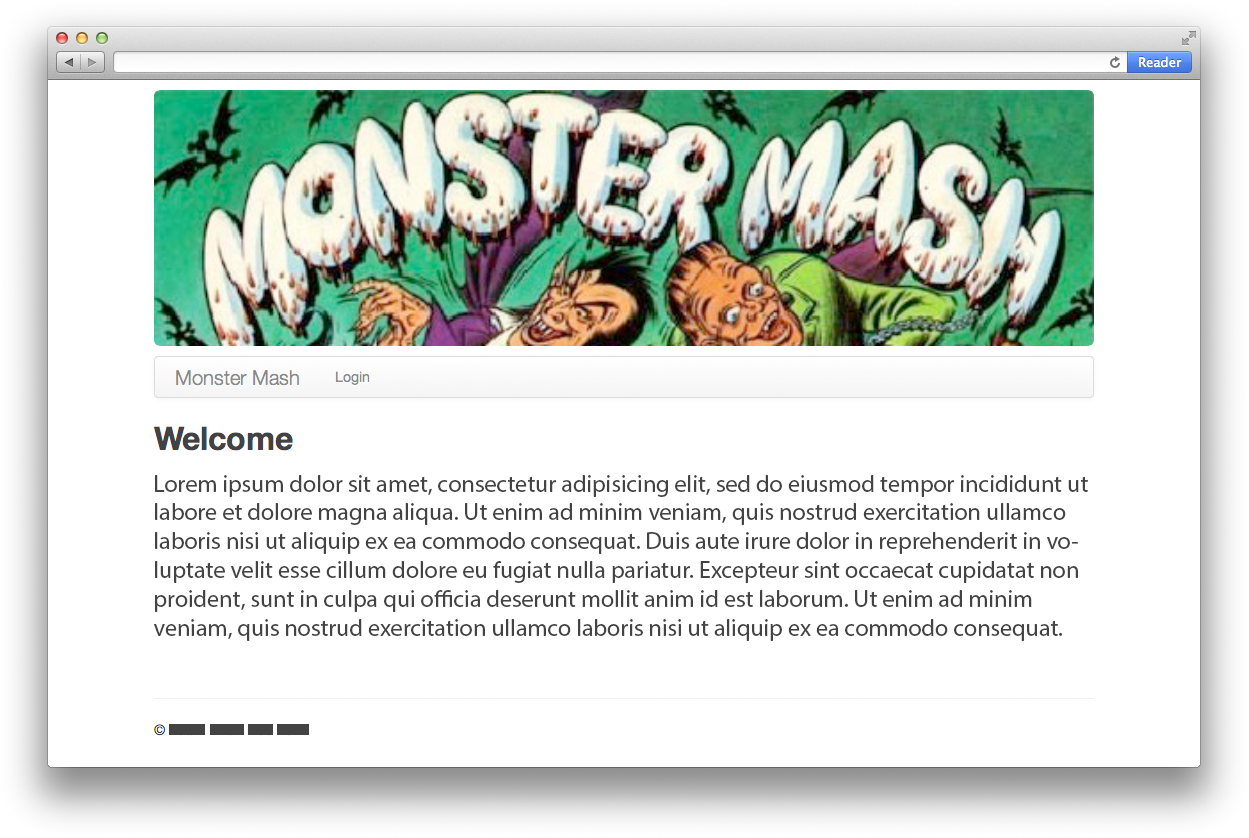
\includegraphics[width=17cm, height=15cm]{index.jpg}
\end{sideways}
\end{figure}
\newpage
\subsection{Login/Register Page}
On this page, a user can login with an existing account or register a new account by clicking on the Register button. This brings up a dialog box on top of the existing page which lets a user register. Upon successful registration they are brought back to the login page so that they can proceed to login.
\begin{figure}[h]
\begin{sideways}
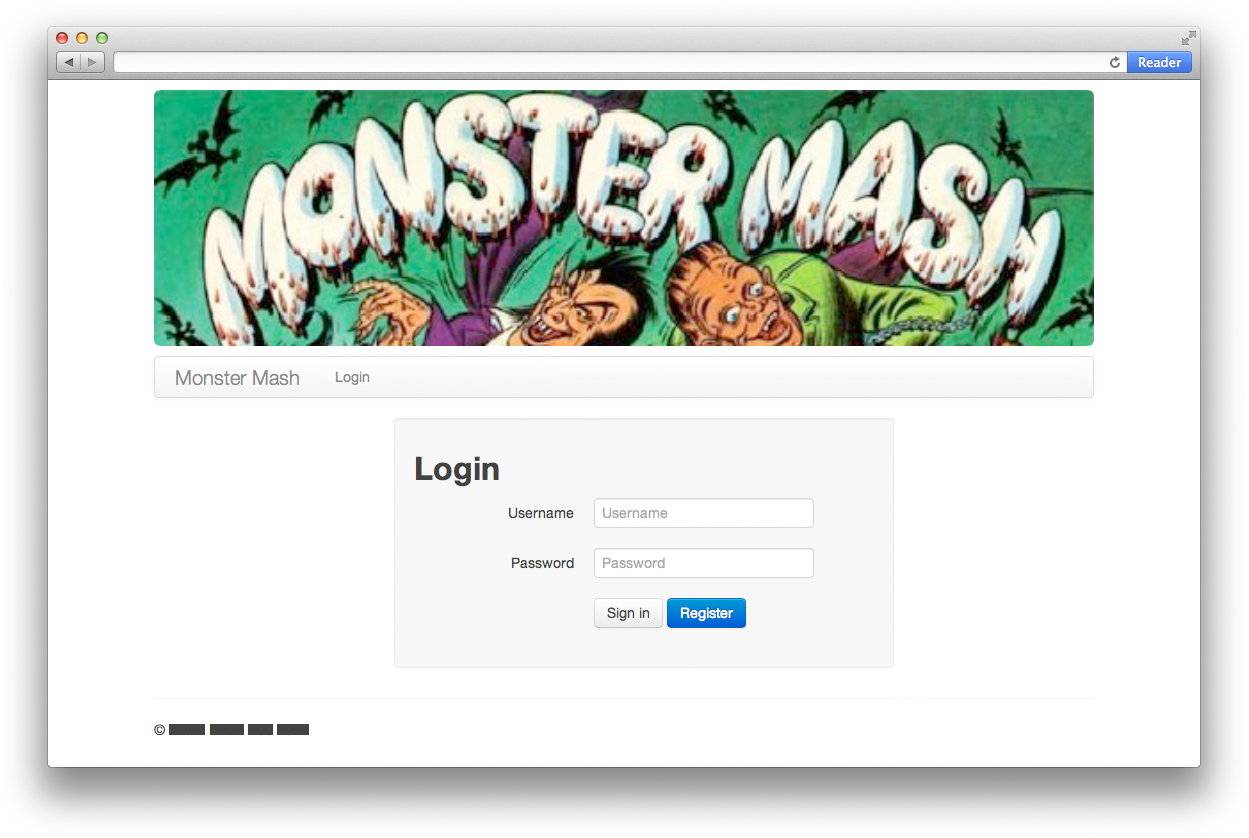
\includegraphics[width=17cm, height=15cm]{login.jpg}
\end{sideways}
\end{figure}
\newpage
\begin{figure}[h]
\begin{sideways}
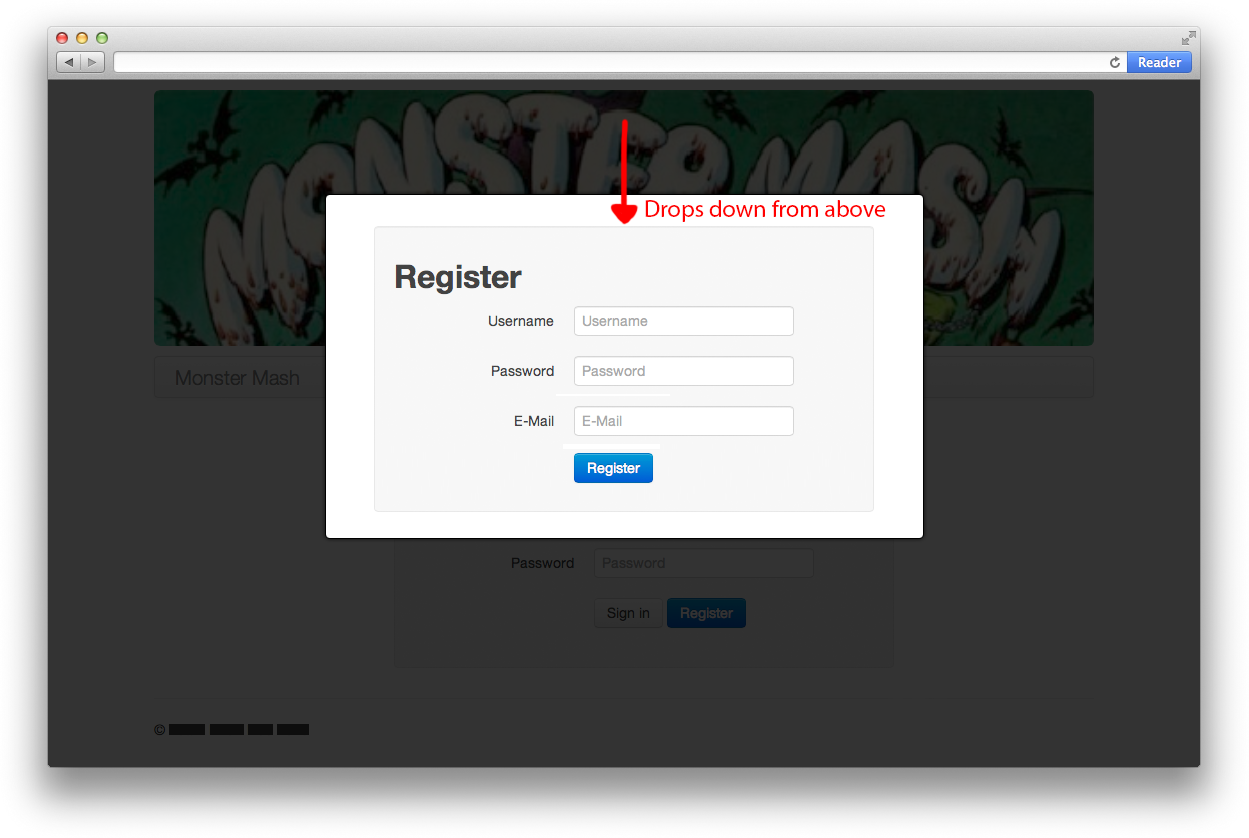
\includegraphics[width=17cm, height=15cm]{register.jpg}
\end{sideways}
\end{figure}
\newpage
\subsection{Home/Add Friend}This is the page a user views once they have logged in. The menu bar now has additional links that a user can follow which indicates to the user they have successfully logged in. On the left it shows their personal user statistics, and their primary monster's statistics. On this page, friend requests, battle requests and other kinds of requests are displayed with an Accept/Decline button. In the bottom right hand corner is a friends list, to bring up the list of friends that a user has. If the user clicks on it, it slides upwards to display all of the user's friends. If they have none, a message to the user is displayed instead and a button to add friends is shown. Upon clicking this, a window slides down with fields to enable the user to add a friend.When typing in the user name box, a list drops down to suggest friend names to add. This list is populated from the user database.
\begin{figure}[h]
\begin{sideways}
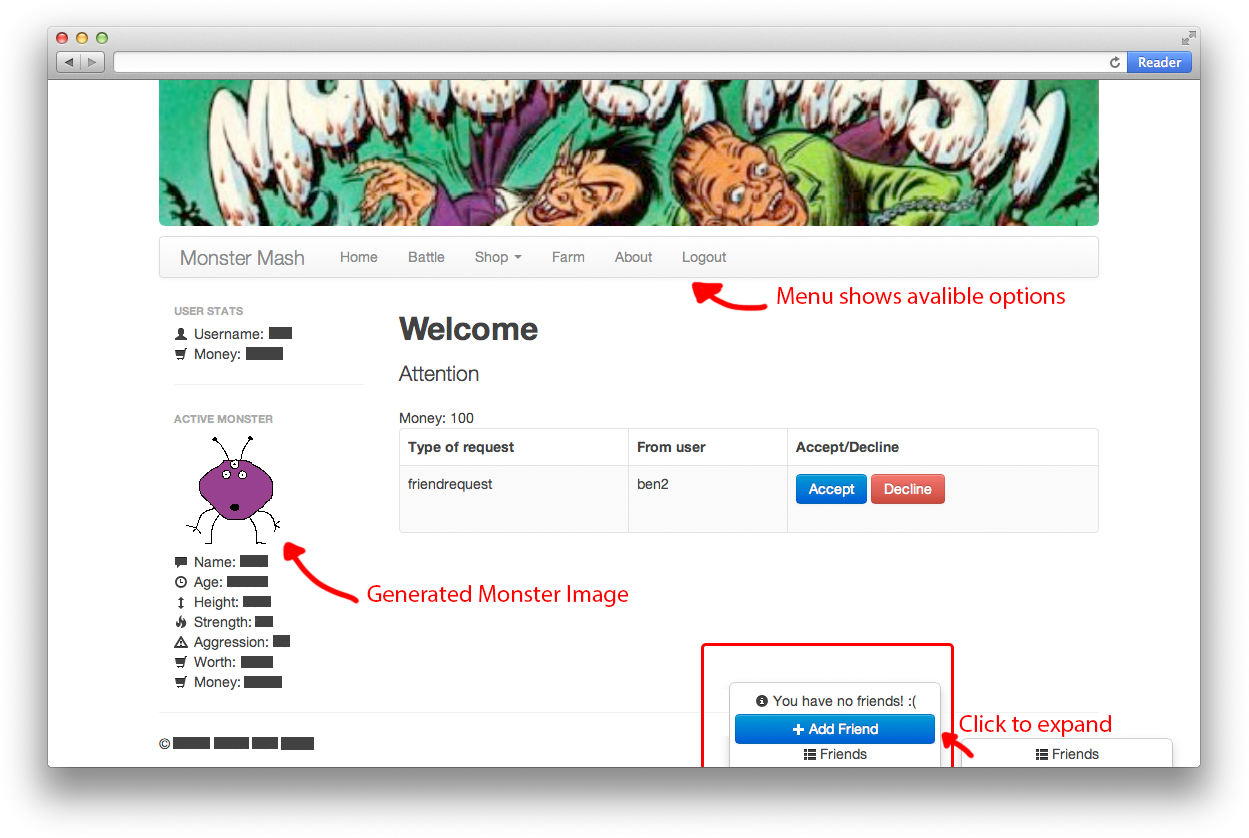
\includegraphics[width=17cm, height=15cm]{home.jpg}
\end{sideways}
\end{figure}
\newpage
\begin{figure}[h]
\begin{sideways}
\includegraphics[width=17cm, height=15cm]{homeaddfriend.jpg}
\end{sideways}
\end{figure}
\newpage
\subsection{Battle Page}
This is the page a user will see when they enter a battle. It shows each monster side by slide, along with their statistics, and has a "Battle" button to initiate the battle.
\begin{figure}[h]
\begin{sideways}
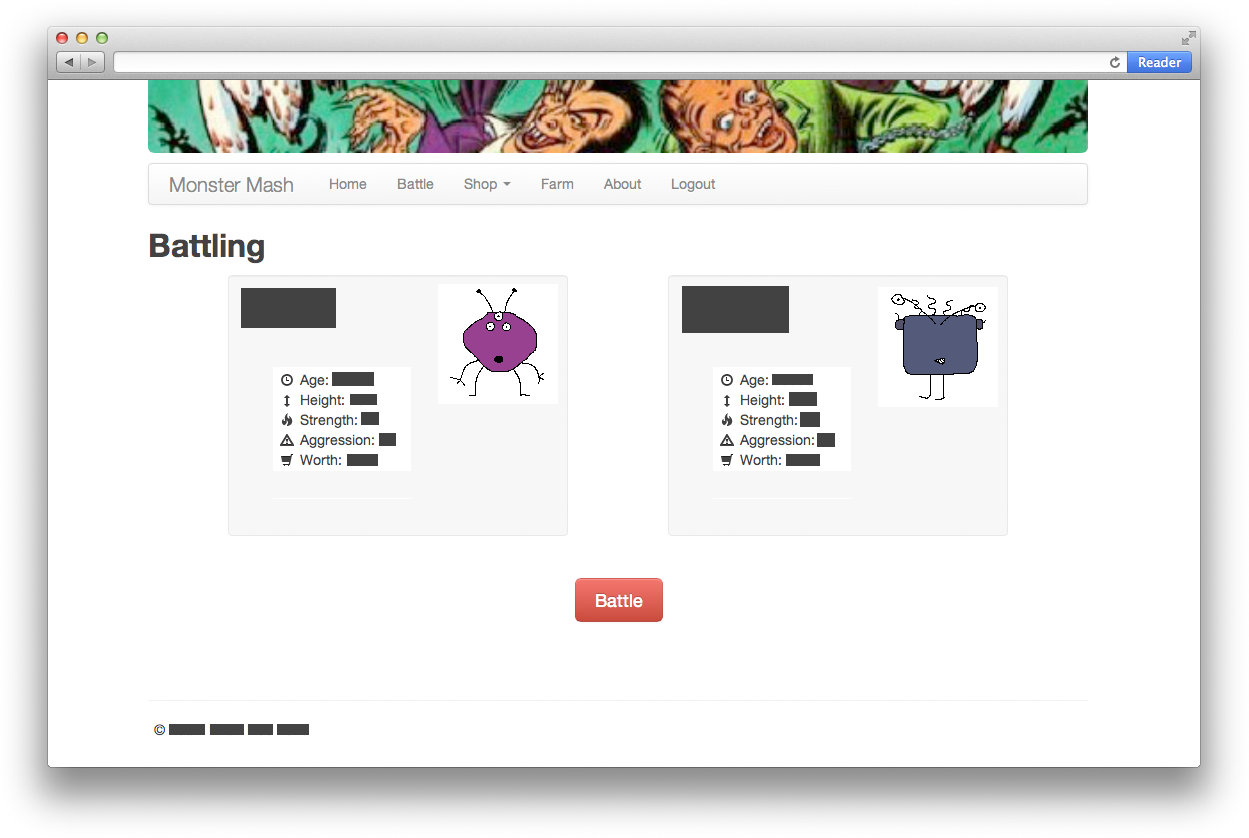
\includegraphics[width=17cm, height=15cm]{battle.jpg}
\end{sideways}
\end{figure}
\newpage
\subsection{Shop Page}
A user can buy or sell monsters in the Monster Shop. Their own monsters will be displayed in a table with an option to sell each of them, or alternatively, a list of unowned monsters can be displayed with an option to buy them. These are automatically added to the shop database when a user creates an account to add populate the Shop. All of the statistics are visible in the table so a user knows what attributes the monster they are buying has.
\begin{figure}[h]
\begin{sideways}
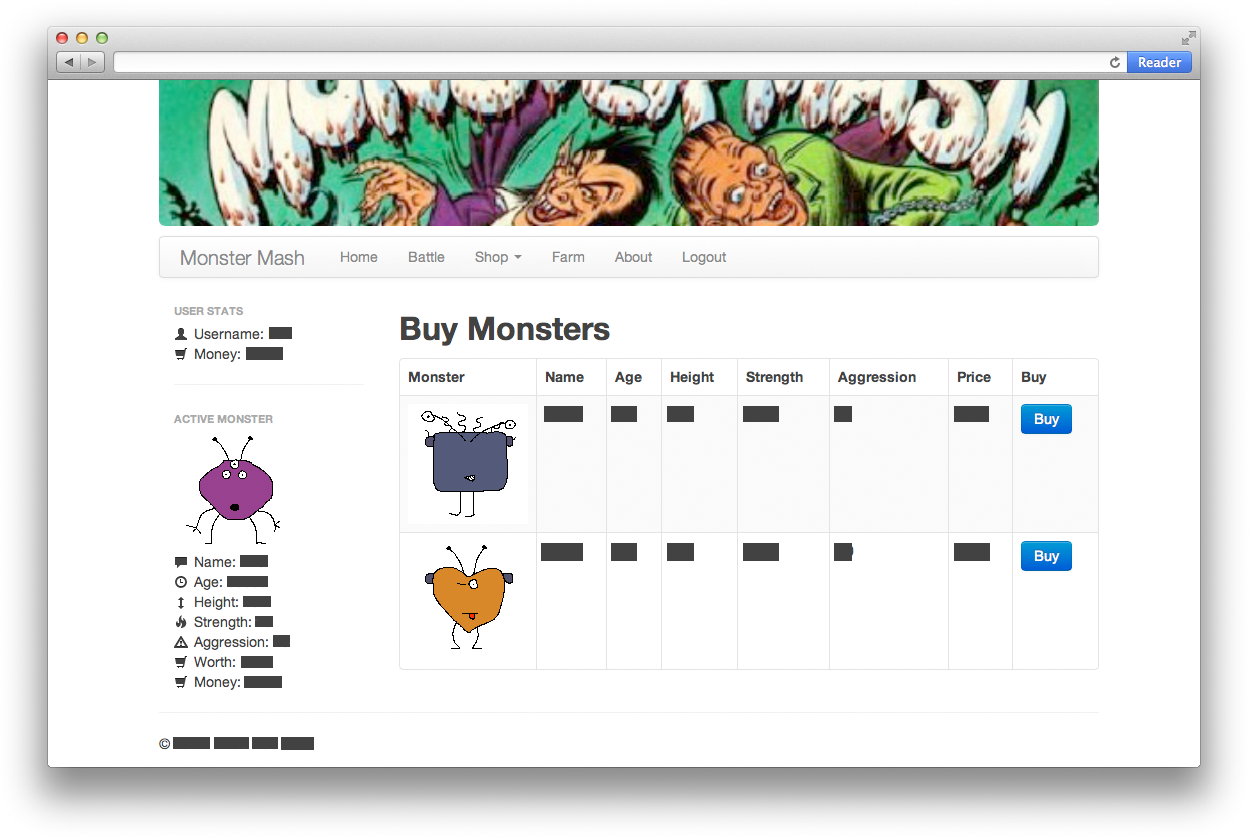
\includegraphics[width=17cm, height=15cm]{shop.jpg}
\end{sideways}
\end{figure}
\newpage
\section{Gantt Chart}
\subsection{Key for Gantt Chart}
\begin{figure*}[h]
\includegraphics[width=1.00\textwidth]{GanntKey.jpg} 
\label{fig:GanntKey}
\end{figure*}
\newpage
\subsection{Gantt Chart}
\begin{figure*}[h]
\begin{sideways}
\includegraphics[width=16cm, height=17cm]{GanttChart.pdf} 
\label{fig:GanttChart}
\end{sideways}
\end{figure*}
\newpage
\section{Risk Analysis}
When planning and developing a piece of Software, there are many different aspects of the development process. This is why Software Engineers need to try and predict and possibility and minimise the chances of problems having any serious effect on the development of an application e.g. - losing time, unable to make a deadline or even to the extent of a particular part of the project being left incomplete or not working.
\newline
Primarily it is the job of the Project Group to identify these risks and to remain committed so that they can be avoided at all costs or at least minimised in regards of damage to development.\\
\\\begin{tabular}{|p{5cm}|p{5cm}|p{5cm}|}
\hline
Description & Possible Outcomes & Actions to take \\
\hline
Time allocation being unrealistic. & Team members unable to finish their work or finish it to the best of their ability. & Plan correctly, ensure that all members are happy that work can be completed in that length of time.\\
\hline
Communication - All members need to have an idea of what they and other group members are doing in terms of development. & Lack of communication can lead to tasks being incomplete. & Smooth running project and deadline being met.\\
\hline
Illness of key group members. & Group members are unsure of what needs to be done. & Deputy Project Manager needs to know what the Project Leader has planned so that they can carry on without major disruption.\\
\hline
Members of the group leaving the project group due to unforeseen circumstances. & This could result in work being left incomplete halfway through, work having to be reassigned to group members by the project leader and slowing down overall progress. & Have a contingency plan in place that can deal with the event of group members leaving. Have a backup project plan which has work already reallocated in the event of a person leaving.\\
\hline
Learning how to use new programs. & Simple tasks may be more time consuming. E.g. in Latex and GitHub. & Use of books and other group members to ensure they understand new technology in a suitable timespace.\\
\hline
Software and Hardware difficulties. & This could result in data and progress being lost and not being able to develop the application effectively. & Have alternative hardware and software options. E.g Personal Computer or other Software. \\
\hline
Difficulty integrating different group members code. & Hard to pull code together and integrating the GUI. & Ensure that coders work closely together so that this problem is mitigated. \\
\hline
Group repository inaccessible/technical difficulties. & Can lead to missed deadlines and lack of development. & All members should backup their own work individually so that these issues have minimal effect. \\
\hline
Complex algorithms. & Can lead to code that contains bugs that are difficult to fix or can't be fixed. & Write small segments of code at a time and then compile. This make it easier compared to a large segment of code being compiled and containing bugs as there is less code to debug. \\
\hline
Inaccessible network. & Leads to lost time within the project. & Saving files locally as well as on server. Also pulling and pushing to Git regularly to ensure latest version is available.\\
\hline
\end{tabular}
\section{References}
[1] Software Engineering Group Project Plan Specification Standards.  Bernard Tiddeman. SE.QA.05B. 1.1 Release
\section{Document History}
\begin{table*}[h]
\caption{Document History}
\centering
\begin{tabular}{|c|c|c|c|c|}
\hline\hline
Version & CCF No.\ & Date \ & Changes made to document\ & Changed by: \\ [0.5ex]
\hline
1.0 & N/A & 25/10/2012 & Creating Project Plan & arj18 \\
\hline
1.1 & N/A  & 29/10/2012 & Making changes from review & arj18 \\
\hline
1.2 & N/A  & 30/10/2012  & Adding final GUI designs & arj18 \\
\hline
1.3 & N/A  & 28/01/2013  & Adding feedback changes to document & arj18  \\ [1ex]	
\hline 
1.4 & N/A & 12/02/2013 & Adding revised GUI designs. & arj8 \\
\hline
1.5 & N/A & 13/02/2013 & Spell Checked and added some Risk Analysis & sam39 \\
\hline
\end{tabular}
\label{table:nonlin}
\end{table*}
\end{document}
